\documentclass[aps,pra,preprint,groupedaddress]{revtex4-1}
\usepackage{graphicx}
\usepackage{setspace}
\usepackage{epsfig}
\usepackage{amsmath}
\usepackage{mathrsfs}
\usepackage{braket}
\usepackage{amssymb} % symbols
\usepackage{mathtools}
\usepackage{graphicx}
\usepackage{textcomp}
\usepackage{amssymb}
%\usepackage{slashbox}
\usepackage{geometry}
\usepackage{subfigure}
\usepackage[normalem]{ulem}
\usepackage{color}
\usepackage{float}

\newcommand{\note}[1]{\textcolor{red}{#1}}
\newcommand{\nn}{\nonumber}



\begin{document}
\center{\textbf{Supporting Information}}\\
\center{\textbf{Polarons Explain Luminescence Behavior of Colloidal Quantum Dots at Low Temperature}}\\
\center{Meenakshi Khosla, Sravya Rao, and Shilpi Gupta}\\


%\maketitle
\bigskip

%Supplementary figure 1
\begin{figure}[htbp]
\renewcommand{\figurename}{\textbf{Figure S}}
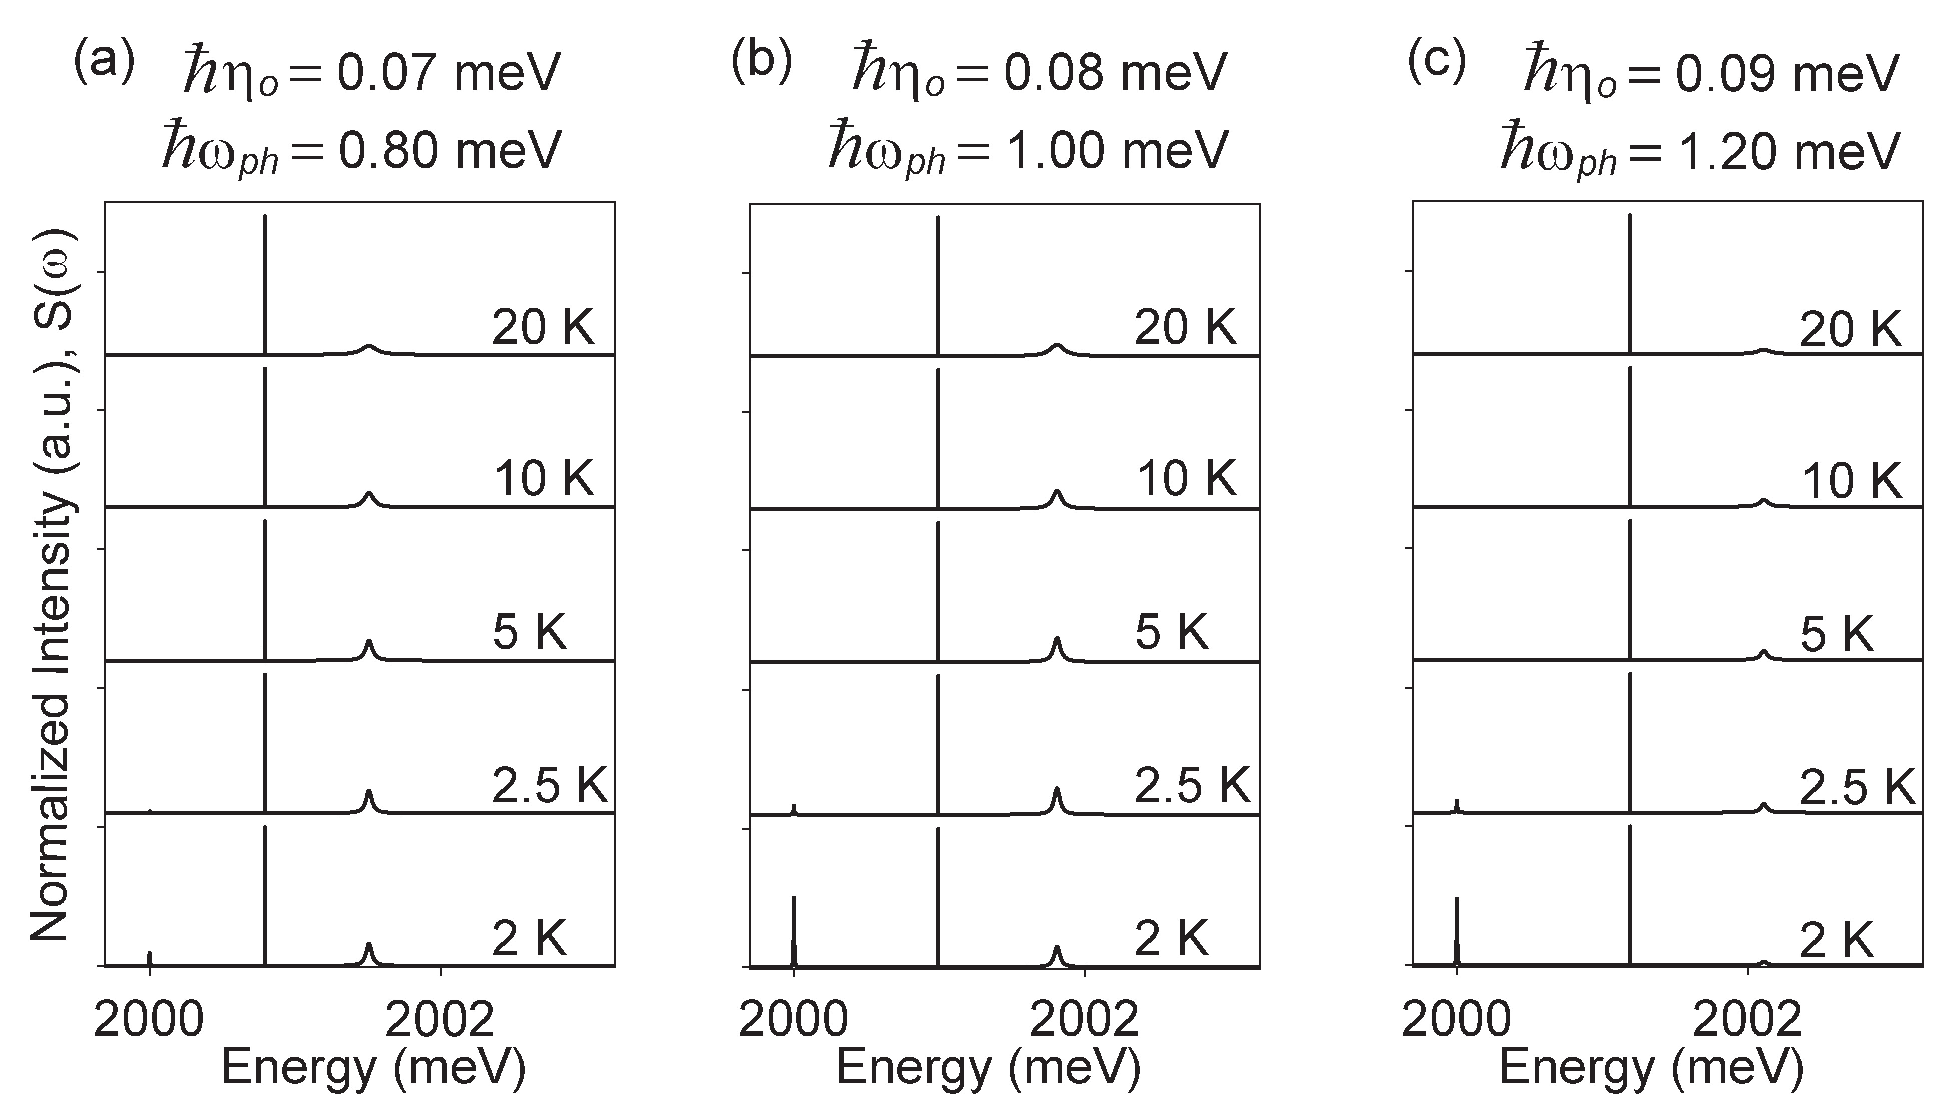
\includegraphics[width=\textwidth]{Supplementary_Fig1.eps}
\caption{Spectrum for different values of $\omega_{ph}$ and $\eta_0$. (a)$\hbar\eta_0 =$ 0.07 meV and $\hbar\omega_{ph} =$ 0.80 meV. (b)$\hbar\eta_0 =$ 0.08 meV and $\hbar\omega_{ph} =$ 1.00 meV.  (c)$\hbar\eta_0 =$ 0.09 meV and $\hbar\omega_{ph} =$ 1.20 meV. Spectral diffusion is not included.}
\label{Fig:Spectrum_extra}
\end{figure}

%Supplementary figure 2
\begin{figure}[htbp]
\renewcommand{\figurename}{\textbf{Figure S}}
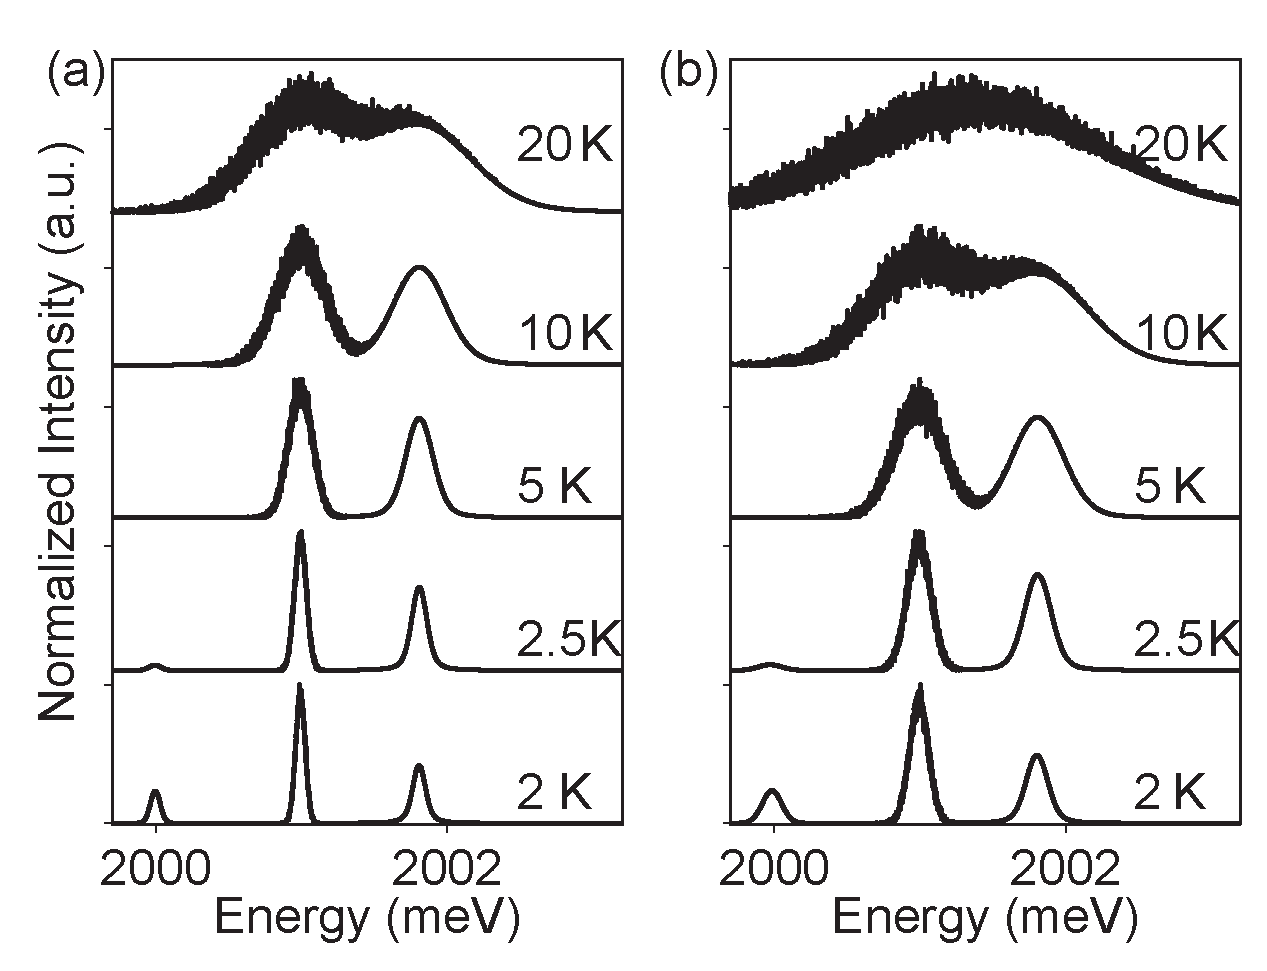
\includegraphics[width= 10 cm]{Supplementary_Fig2.eps}
\caption{Spectrum including spectral diffusion as a Gaussian distribution with standard deviation varying linearly with temperature $T$. Standard deviation (a) 4$T$ ns$^{-1}$. (b) 8$T$ ns$^{-1}$.}
\label{Fig:Spectrum_extra_SpectralDiffusion_Linear}
\end{figure}

%Supplementary figure 3
\begin{figure}[htbp]
\renewcommand{\figurename}{\textbf{Figure S}}
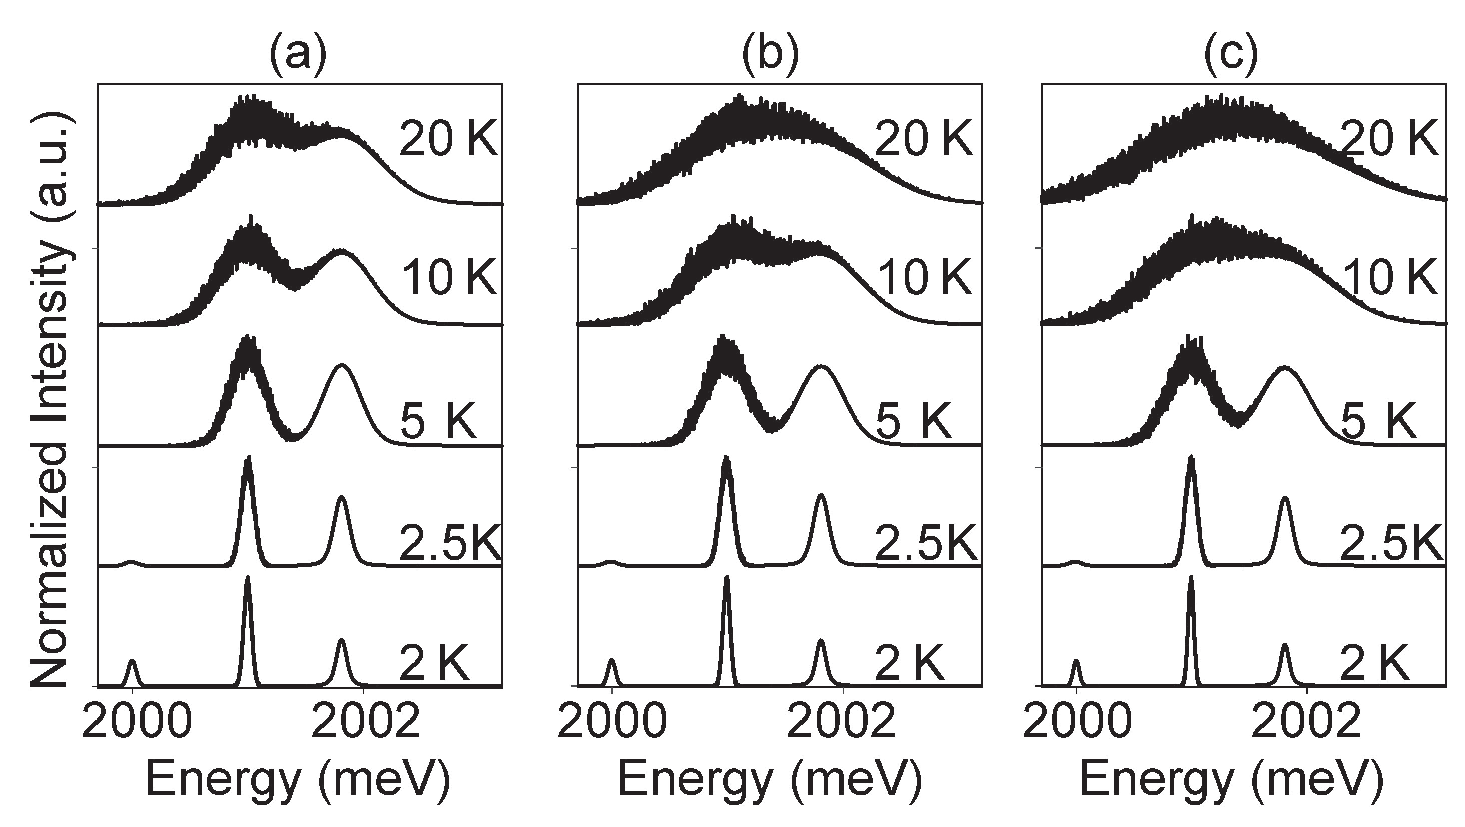
\includegraphics[width=12 cm]{Supplementary_Fig3.eps}
\caption{Spectrum including spectral diffusion as a Gaussian distribution with standard deviation varying with temperature $T$ as Boltzmann Distribution. Standard deviation (a) 100e$^{-5/T}$ ns$^{-1}$. (b) 150e$^{-6/T}$ ns$^{-1}$.  (c) 200e$^{-7/T}$ ns$^{-1}$.}
\label{Fig:Spectrum_extra_SpectralDiffusion_exp}
\end{figure}

%Supplementary figure 4
\begin{figure}[htbp]
\renewcommand{\figurename}{\textbf{Figure S}}
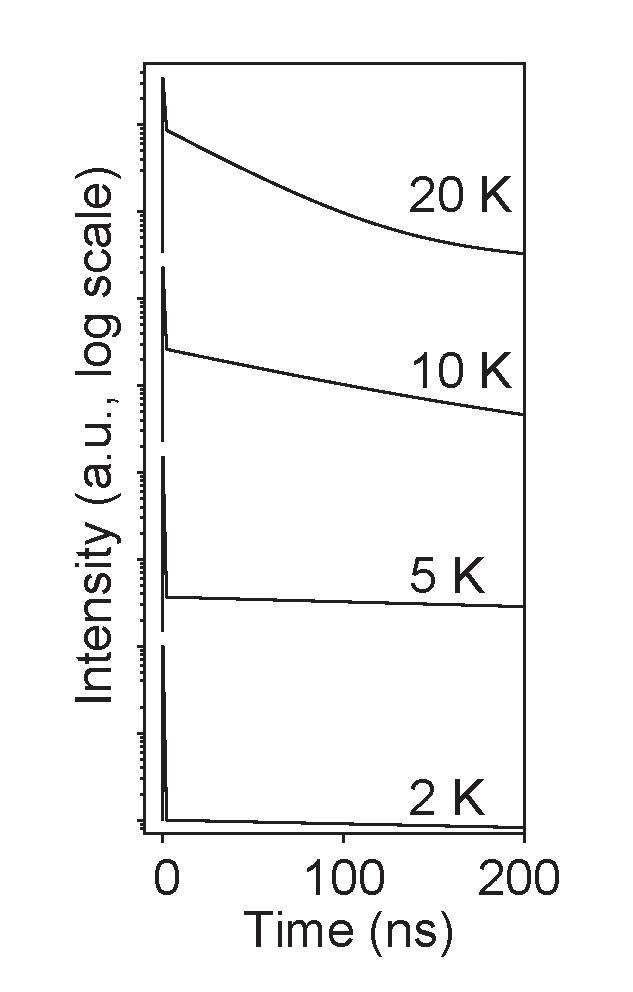
\includegraphics[width= 5cm]{Supplementary_Fig4.eps}
\caption{Decay curves for a different set of initial conditions. $\rho_{++}(0) = 0.5, \rho_{--}(0) = 0.5, \rho_{11}(0) = 0$.}
\label{Fig:Lifetime_extra}
\end{figure}

\end{document}